\section{Технический проект}
\subsection{Общая характеристика организации решения задачи}

Необходимо спроектировать и разработать веб-платформу, направленную на продвижение и оптимизацию деятельности компании на рынке.

Интернет-платформа представляет собой совокупность взаимосвязанных веб-сервисов, доступных через единый пользовательский интерфейс. Каждый сервис представляет собой отдельный функциональный модуль, содержащий текстовую, графическую, а также мультимедийную информацию (видеоконференции, изображения, файлы и т.д.).

Веб-платформа и её веб-сервисы будут размещены в сети Интернет по определённому доменному имени (например, https://calendar.mycompany.ru, https://talks.mycompany.ru, https://mail.mycompany.ru и т.д.). Каждая страница платформы реализуется с использованием современных веб-технологий: HTML, CSS, JavaScript (React) и других, а также может использовать фреймворки и библиотеки для обеспечения адаптивности, интерактивности и высокой производительности.

\subsection{Обоснование выбора технологии проектирования}

На сегодняшний день информационный рынок, поставляющий программные решения в выбранной сфере, предлагает множество продуктов, позволяющих достигнуть поставленной цели – разработки веб-платформы.

\subsubsection{Описание используемых языков программирования}

В процессе разработки веб-платформы используются программные средства и языки программирования. Каждое программное средство и каждый язык программирования применяется для круга задач, при решении которых они необходимы.

\subsubsection{Язык программирования Python}

Python — это высокоуровневый язык программирования общего назначения с поддержкой нескольких парадигм, включая объектно-ориентированное, процедурное и функциональное программирование. Благодаря своей простоте, читаемости и обширной экосистеме библиотек, Python широко применяется в разработке веб-приложений, автоматизации процессов, анализе данных, машинном обучении и многих других областях. В контексте разработки веб-приложений Python используется совместно с фреймворками, такими как Django и Flask, которые обеспечивают удобные средства для создания серверной логики, обработки запросов и генерации динамических веб-страниц.

\subsubsection{Язык программирования TypeScript}

TypeScript — это высокоуровневый интерпретируемый язык программирования, основной задачей которого является создание интерактивного поведения на веб-страницах, с поддержкой жёсткой типизации. Он является неотъемлемой частью технологии разработки клиентской части веб-приложений и поддерживается всеми современными веб-браузерами. С помощью TypeScript можно реализовывать динамическое обновление содержимого, проверку данных на стороне клиента, обработку событий, а также взаимодействие с сервером без перезагрузки страницы (через AJAX-запросы). Современные стандарты TypeScript предоставляют широкий набор возможностей, включая модули, асинхронные функции, классы и работу с промисами. Для повышения совместимости и ускорения разработки часто используются библиотеки и фреймворки, такие как jQuery, React, Vue.js и другие. Они позволяют упростить доступ к элементам DOM, реализовать реактивные интерфейсы и обеспечить кроссбраузерную поддержку. JavaScript выполняется непосредственно в браузере пользователя, что позволяет создавать отзывчивые и интерактивные пользовательские интерфейсы без необходимости постоянной связи с сервером.

\subsubsection{React}
React — это популярная JavaScript-библиотека для создания пользовательских интерфейсов. Она позволяет строить интерактивные веб-приложения с помощью компонентного подхода.

Основные преимущества React:
\begin{enumerate}
\item Виртуальный DOM для эффективного обновления интерфейса.
\item Компонентная архитектура, способствующая повторному использованию кода.
\item Односторонний поток данных, упрощающий отладку приложений.
\item Богатая экосистема дополнительных библиотек и инструментов.
\item Поддержка серверного рендеринга (Next.js).
\end{enumerate}

В нашем проекте React используется для построения клиентской части всех веб-сервисов платформы. Это позволяет создавать единообразные, отзывчивые интерфейсы с высокой производительностью.

\subsubsection{Apache James и JMAP}
Apache James — это open-source почтовый сервер, написанный на Java. Он предоставляет полный набор почтовых протоколов (SMTP, POP3, IMAP) и может использоваться как самостоятельное решение или как часть более крупной системы.

JMAP (JSON Meta Application Protocol) — современный протокол для работы с почтой, календарями и контактами, призванный заменить устаревшие IMAP и SMTP. Его преимущества:
\begin{itemize}
\item использование JSON для передачи данных;
\item эффективная синхронизация состояния;
\item поддержка push-уведомлений;
\item единый API для почты, календарей и контактов.
\end{itemize}

В нашей платформе мы используем Apache James с поддержкой JMAP для реализации почтового сервиса, что обеспечивает:
\begin{itemize}
\item надежную доставку и хранение почты;
\item быструю синхронизацию между клиентами;
\item современный API для интеграции с другими сервисами.
\end{itemize}

\subsubsection{Node.js}
Node.js — это серверная платформа для выполнения JavaScript, построенная на движке V8. Она использует событийно-ориентированную, неблокирующую модель ввода-вывода, что делает её легковесной и эффективной.

Основные особенности Node.js, используемые в нашем проекте:
\begin{itemize}
\item высокая производительность для I/O-интенсивных операций;
\item единая языковая среда для клиента и сервера (JavaScript);
\item богатая экосистема пакетов (npm);
\item поддержка современных стандартов JavaScript.
\end{itemize}

В нашей архитектуре Node.js используется для:
\begin{itemize}
\item реализации серверной логики некоторых микросервисов;
\item обработки реального времени (чаты, уведомления);
\item серверного рендеринга React-приложений;
\item построения API-шлюза для объединения различных сервисов.
\end{itemize}

Сочетание этих технологий позволяет нам создать масштабируемую, производительную платформу с современным пользовательским интерфейсом и надежной серверной частью.

\subsection{Диаграмма компонентов}

Диаграмма компонентов в UML (Unified Modeling Language) — это структурная диаграмма, которая отображает состав и взаимодействие компонентов системы на высоком уровне абстракции. На рисунке  ~\ref{comp:image} представлена диаграмма компонентов для проектируемой системы.

\begin{figure}[H]
\center{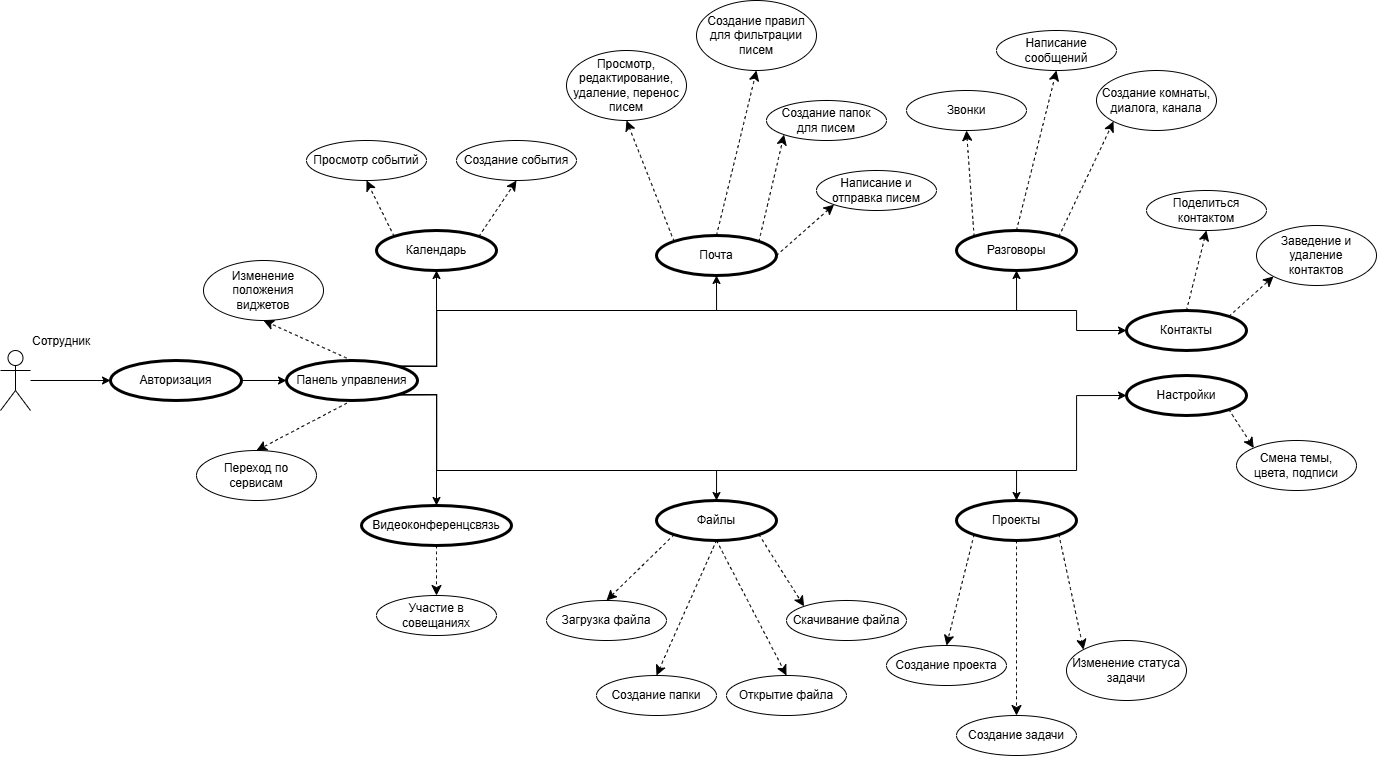
\includegraphics[width=0.7\linewidth]{images/diag2}}
\caption{Диаграмма компонентов}
\label{comp:image}
\end{figure}

\subsection{Структура базы данных}

Сущности и отношение между таблицами базы данных отражены на рисунке \ref{place:image}

\begin{figure}[H]
\center{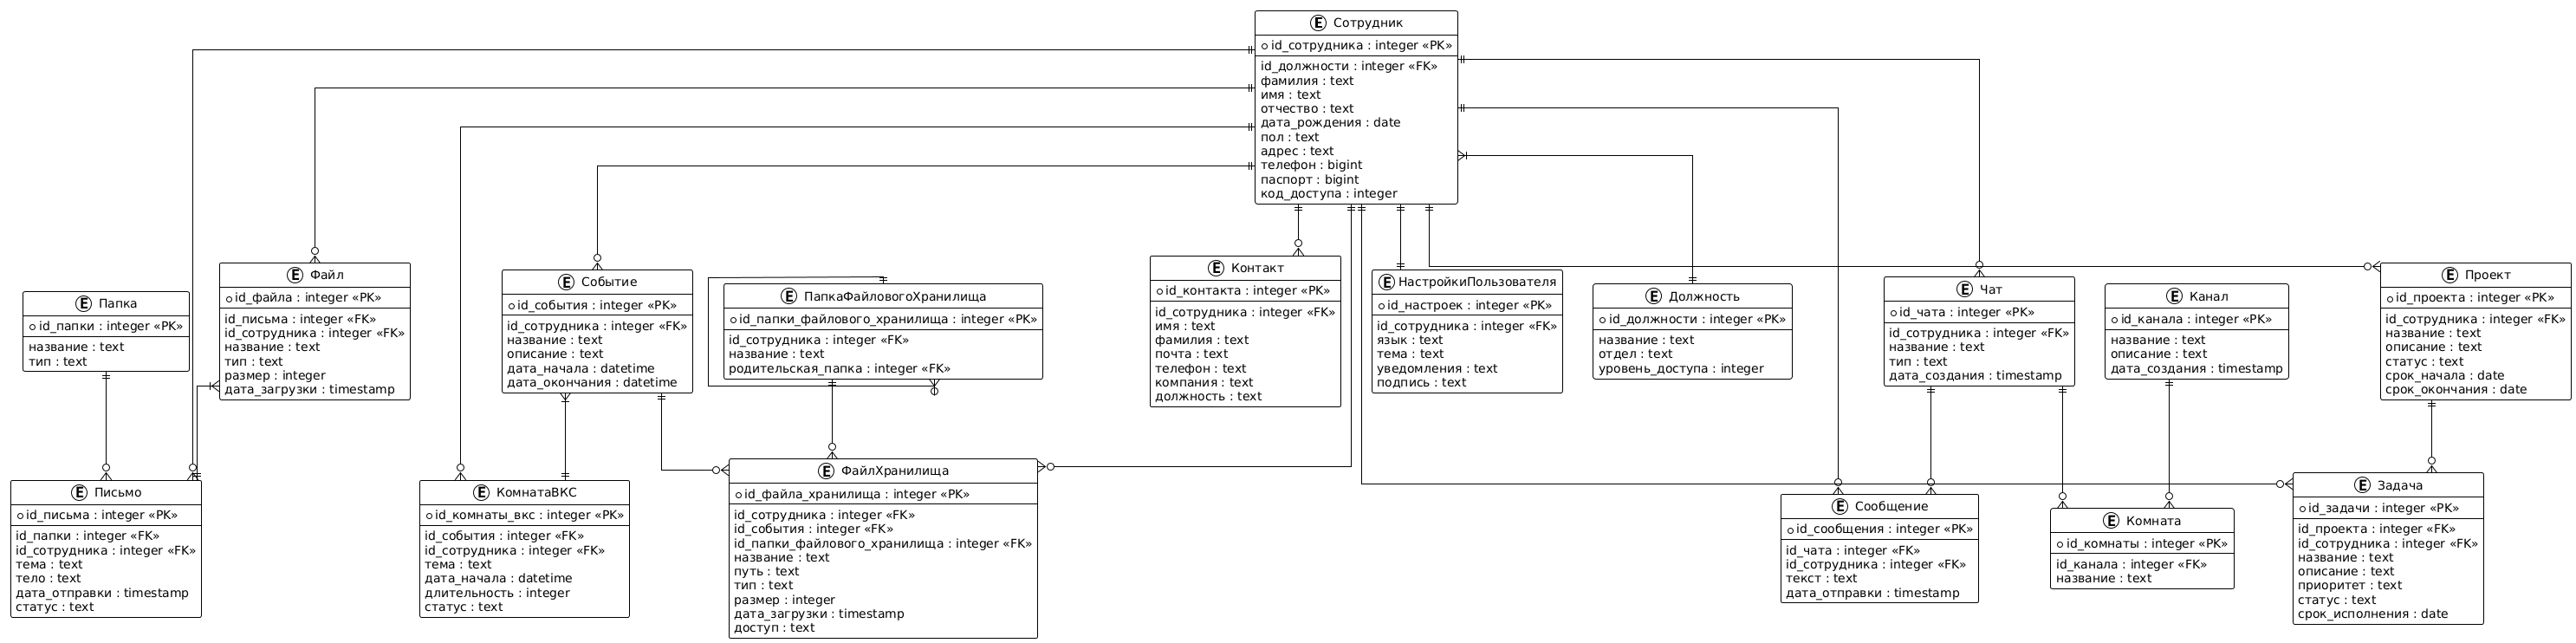
\includegraphics[width=1\linewidth]{images/erdiag}}
\caption{ER-диаграмма}
\label{place:image}
\end{figure}

В таблице \ref{employee:table} представлена структура таблицы employee. Таблица содержит данные о сотрудниках: уникальный идентификатор, идентификатор должности, фамилия, имя, отчество, дата рождения, пол, адрес, телефон, паспорт и код доступа.

\begin{xltabular}{\textwidth}{|l|p{5cm}|p{3cm}|X|}
  \caption{Таблица employee\label{employee:table}} \\ \hline
  \centrow Тип ключа & \centrow Имя столбца & \centrow Тип данных & \centrow Обязательность \\ \hline
  \endfirsthead
  \continuecaption{Продолжение таблицы \ref{employee:table}}
  \centrow Тип ключа & \centrow Имя столбца & \centrow Тип данных & \centrow Обязательность \\ \hline
  \finishhead
  primary key & id\_employee & Integer & true \\ \hline
  foreign key & id\_position & Integer & true \\ \hline
  ~ & last\_name & Text & true \\ \hline
  ~ & first\_name & Text & true \\ \hline
  ~ & middle\_name & Text & false \\ \hline
  ~ & birth\_date & Date & true \\ \hline
  ~ & gender & Text & true \\ \hline
  ~ & address & Text & false \\ \hline
  ~ & phone\_number & Bigint & true \\ \hline
  ~ & passport\_number & Bigint & false \\ \hline
  ~ & access\_code & Integer & true \\ \hline
\end{xltabular}


В таблице \ref{position:table} представлена структура таблицы position. Таблица содержит данные о должностях: уникальный идентификатор, название должности, отдел и уровень доступа.

\begin{xltabular}{\textwidth}{|l|p{5cm}|p{3cm}|X|}
  \caption{Таблица position\label{position:table}} \\ \hline
  \centrow Тип ключа & \centrow Имя столбца & \centrow Тип данных & \centrow Обязательность \\ \hline
  \endfirsthead
  \continuecaption{Продолжение таблицы \ref{position:table}}
  \centrow Тип ключа & \centrow Имя столбца & \centrow Тип данных & \centrow Обязательность \\ \hline
  \finishhead
  primary key & id\_position & Integer & true \\ \hline
  ~ & name & Text & true \\ \hline
  ~ & department & Text & true \\ \hline
  ~ & access\_level & Integer & true \\ \hline
\end{xltabular}


В таблице \ref{project:table} представлена структура таблицы project. Таблица содержит данные о проектах: уникальный идентификатор, идентификатор сотрудника (руководителя), название, описание, статус, дата начала и окончания.

\begin{xltabular}{\textwidth}{|l|p{5cm}|p{3cm}|X|}
  \caption{Таблица project\label{project:table}} \\ \hline
  \centrow Тип ключа & \centrow Имя столбца & \centrow Тип данных & \centrow Обязательность \\ \hline
  \endfirsthead
  \continuecaption{Продолжение таблицы \ref{project:table}}
  \centrow Тип ключа & \centrow Имя столбца & \centrow Тип данных & \centrow Обязательность \\ \hline
  \finishhead
  primary key & id\_project & Integer & true \\ \hline
  foreign key & id\_employee & Integer & true \\ \hline
  ~ & name & Text & true \\ \hline
  ~ & description & Text & false \\ \hline
  ~ & status & Text & true \\ \hline
  ~ & start\_date & Date & true \\ \hline
  ~ & end\_date & Date & true \\ \hline
\end{xltabular}


В таблице \ref{task:table} представлена структура таблицы task. Таблица содержит данные о задачах: уникальный идентификатор, идентификатор проекта, идентификатор исполнителя, название, описание, приоритет, статус и срок исполнения.

\begin{xltabular}{\textwidth}{|l|p{5cm}|p{3cm}|X|}
  \caption{Таблица task\label{task:table}} \\ \hline
  \centrow Тип ключа & \centrow Имя столбца & \centrow Тип данных & \centrow Обязательность \\ \hline
  \endfirsthead
  \continuecaption{Продолжение таблицы \ref{task:table}}
  \centrow Тип ключа & \centrow Имя столбца & \centrow Тип данных & \centrow Обязательность \\ \hline
  \finishhead
  primary key & id\_task & Integer & true \\ \hline
  foreign key & id\_project & Integer & true \\ \hline
  foreign key & id\_employee & Integer & true \\ \hline
  ~ & name & Text & true \\ \hline
  ~ & description & Text & false \\ \hline
  ~ & priority & Text & true \\ \hline
  ~ & status & Text & true \\ \hline
  ~ & due\_date & Date & true \\ \hline
\end{xltabular}


В таблице \ref{filefolder:table} представлена структура таблицы file\_storage\_folder. Таблица содержит данные о папках файлового хранилища: уникальный идентификатор, идентификатор владельца, название и родительскую папку.

\begin{xltabular}{\textwidth}{|l|p{5cm}|p{3cm}|X|}
  \caption{Таблица file\_storage\_folder\label{filefolder:table}} \\ \hline
  \centrow Тип ключа & \centrow Имя столбца & \centrow Тип данных & \centrow Обязательность \\ \hline
  \endfirsthead
  \continuecaption{Продолжение таблицы \ref{filefolder:table}}
  \centrow Тип ключа & \centrow Имя столбца & \centrow Тип данных & \centrow Обязательность \\ \hline
  \finishhead
  primary key & id\_file\_storage\_folder & Integer & true \\ \hline
  foreign key & id\_employee & Integer & true \\ \hline
  ~ & name & Text & true \\ \hline
  foreign key & parent\_folder & Integer & false \\ \hline
\end{xltabular}


В таблице \ref{folder:table} представлена структура таблицы folder. Таблица содержит данные о папках почты и других сервисов: уникальный идентификатор, название и тип.

\begin{xltabular}{\textwidth}{|l|p{5cm}|p{3cm}|X|}
  \caption{Таблица folder\label{folder:table}} \\ \hline
  \centrow Тип ключа & \centrow Имя столбца & \centrow Тип данных & \centrow Обязательность \\ \hline
  \endfirsthead
  \continuecaption{Продолжение таблицы \ref{folder:table}}
  \centrow Тип ключа & \centrow Имя столбца & \centrow Тип данных & \centrow Обязательность \\ \hline
  \finishhead
  primary key & id\_folder & Integer & true \\ \hline
  ~ & name & Text & true \\ \hline
  ~ & type & Text & true \\ \hline
\end{xltabular}


В таблице \ref{letter:table} представлена структура таблицы letter. Таблица содержит данные о письмах: уникальный идентификатор, идентификатор папки, идентификатор отправителя, тема, тело письма, дата отправки и статус.

\begin{xltabular}{\textwidth}{|l|p{5cm}|p{3cm}|X|}
  \caption{Таблица letter\label{letter:table}} \\ \hline
  \centrow Тип ключа & \centrow Имя столбца & \centrow Тип данных & \centrow Обязательность \\ \hline
  \endfirsthead
  \continuecaption{Продолжение таблицы \ref{letter:table}}
  \centrow Тип ключа & \centrow Имя столбца & \centrow Тип данных & \centrow Обязательность \\ \hline
  \finishhead
  primary key & id\_letter & Integer & true \\ \hline
  foreign key & id\_folder & Integer & true \\ \hline
  foreign key & id\_employee & Integer & true \\ \hline
  ~ & subject & Text & true \\ \hline
  ~ & body & Text & false \\ \hline
  ~ & sent\_date & Timestamp & true \\ \hline
  ~ & status & Text & true \\ \hline
\end{xltabular}


В таблице \ref{file:table} представлена структура таблицы file. Таблица содержит данные о файлах: уникальный идентификатор, идентификатор письма, идентификатор сотрудника (загрузившего), название, тип, размер и дату загрузки.

\begin{xltabular}{\textwidth}{|l|p{5cm}|p{3cm}|X|}
  \caption{Таблица file\label{file:table}} \\ \hline
  \centrow Тип ключа & \centrow Имя столбца & \centrow Тип данных & \centrow Обязательность \\ \hline
  \endfirsthead
  \continuecaption{Продолжение таблицы \ref{file:table}}
  \centrow Тип ключа & \centrow Имя столбца & \centrow Тип данных & \centrow Обязательность \\ \hline
  \finishhead
  primary key & id\_file & Integer & true \\ \hline
  foreign key & id\_letter & Integer & true \\ \hline
  foreign key & id\_employee & Integer & true \\ \hline
  ~ & name & Text & true \\ \hline
  ~ & type & Text & true \\ \hline
  ~ & size & Integer & true \\ \hline
  ~ & upload\_date & Timestamp & true \\ \hline
\end{xltabular}


В таблице \ref{event:table} представлена структура таблицы event. Таблица содержит данные о событиях: уникальный идентификатор, идентификатор сотрудника (организатора), название, описание, дата начала и окончания.

\begin{xltabular}{\textwidth}{|l|p{5cm}|p{3cm}|X|}
  \caption{Таблица event\label{event:table}} \\ \hline
  \centrow Тип ключа & \centrow Имя столбца & \centrow Тип данных & \centrow Обязательность \\ \hline
  \endfirsthead
  \continuecaption{Продолжение таблицы \ref{event:table}}
  \centrow Тип ключа & \centrow Имя столбца & \centrow Тип данных & \centrow Обязательность \\ \hline
  \finishhead
  primary key & id\_event & Integer & true \\ \hline
  foreign key & id\_employee & Integer & true \\ \hline
  ~ & name & Text & true \\ \hline
  ~ & description & Text & false \\ \hline
  ~ & start\_date & Datetime & true \\ \hline
  ~ & end\_date & Datetime & true \\ \hline
\end{xltabular}


В таблице \ref{vksroom:table} представлена структура таблицы vks\_room. Таблица содержит данные о комнатах ВКС: уникальный идентификатор, идентификатор события, идентификатор сотрудника (организатора), тема, дата начала, длительность и статус.

\begin{xltabular}{\textwidth}{|l|p{5cm}|p{3cm}|X|}
  \caption{Таблица vks\_room\label{vksroom:table}} \\ \hline
  \centrow Тип ключа & \centrow Имя столбца & \centrow Тип данных & \centrow Обязательность \\ \hline
  \endfirsthead
  \continuecaption{Продолжение таблицы \ref{vksroom:table}}
  \centrow Тип ключа & \centrow Имя столбца & \centrow Тип данных & \centrow Обязательность \\ \hline
  \finishhead
  primary key & id\_vks\_room & Integer & true \\ \hline
  foreign key & id\_event & Integer & true \\ \hline
  foreign key & id\_employee & Integer & true \\ \hline
  ~ & subject & Text & true \\ \hline
  ~ & start\_date & Datetime & true \\ \hline
  ~ & duration & Integer & true \\ \hline
  ~ & status & Text & true \\ \hline
\end{xltabular}


В таблице \ref{chat:table} представлена структура таблицы chat. Таблица содержит данные о чатах: уникальный идентификатор, идентификатор сотрудника (создателя), название, тип и дата создания.

\begin{xltabular}{\textwidth}{|l|p{5cm}|p{3cm}|X|}
  \caption{Таблица chat\label{chat:table}} \\ \hline
  \centrow Тип ключа & \centrow Имя столбца & \centrow Тип данных & \centrow Обязательность \\ \hline
  \endfirsthead
  \continuecaption{Продолжение таблицы \ref{chat:table}}
  \centrow Тип ключа & \centrow Имя столбца & \centrow Тип данных & \centrow Обязательность \\ \hline
  \finishhead
  primary key & id\_chat & Integer & true \\ \hline
  foreign key & id\_employee & Integer & true \\ \hline
  ~ & name & Text & true \\ \hline
  ~ & type & Text & true \\ \hline
  ~ & creation\_date & Timestamp & true \\ \hline
\end{xltabular}


В таблице \ref{message:table} представлена структура таблицы message. Таблица содержит данные о сообщениях: уникальный идентификатор, идентификатор чата, идентификатор отправителя, текст и дату отправки.

\begin{xltabular}{\textwidth}{|l|p{5cm}|p{3cm}|X|}
  \caption{Таблица message\label{message:table}} \\ \hline
  \centrow Тип ключа & \centrow Имя столбца & \centrow Тип данных & \centrow Обязательность \\ \hline
  \endfirsthead
  \continuecaption{Продолжение таблицы \ref{message:table}}
  \centrow Тип ключа & \centrow Имя столбца & \centrow Тип данных & \centrow Обязательность \\ \hline
  \finishhead
  primary key & id\_message & Integer & true \\ \hline
  foreign key & id\_chat & Integer & true \\ \hline
  foreign key & id\_employee & Integer & true \\ \hline
  ~ & text & Text & true \\ \hline
  ~ & sent\_date & Timestamp & true \\ \hline
\end{xltabular}


В таблице \ref{channel:table} представлена структура таблицы channel. Таблица содержит данные о каналах: уникальный идентификатор, название, описание и дату создания.

\begin{xltabular}{\textwidth}{|l|p{5cm}|p{3cm}|X|}
  \caption{Таблица channel\label{channel:table}} \\ \hline
  \centrow Тип ключа & \centrow Имя столбца & \centrow Тип данных & \centrow Обязательность \\ \hline
  \endfirsthead
  \continuecaption{Продолжение таблицы \ref{channel:table}}
  \centrow Тип ключа & \centrow Имя столбца & \centrow Тип данных & \centrow Обязательность \\ \hline
  \finishhead
  primary key & id\_channel & Integer & true \\ \hline
  ~ & name & Text & true \\ \hline
  ~ & description & Text & false \\ \hline
  ~ & creation\_date & Timestamp & true \\ \hline
\end{xltabular}


В таблице \ref{room:table} представлена структура таблицы room. Таблица содержит данные о комнатах: уникальный идентификатор, идентификатор канала, название.

\begin{xltabular}{\textwidth}{|l|p{5cm}|p{3cm}|X|}
  \caption{Таблица room\label{room:table}} \\ \hline
  \centrow Тип ключа & \centrow Имя столбца & \centrow Тип данных & \centrow Обязательность \\ \hline
  \endfirsthead
  \continuecaption{Продолжение таблицы \ref{room:table}}
  \centrow Тип ключа & \centrow Имя столбца & \centrow Тип данных & \centrow Обязательность \\ \hline
  \finishhead
  primary key & id\_room & Integer & true \\ \hline
  foreign key & id\_channel & Integer & true \\ \hline
  ~ & name & Text & true \\ \hline
\end{xltabular}


В таблице \ref{filestoragefile:table} представлена структура таблицы filestorage\_file. Таблица содержит данные о файлах файлового хранилища: уникальный идентификатор, идентификатор сотрудника (владельца), идентификатор события, идентификатор папки файлового хранилища, название, путь, тип, размер, дату загрузки и права доступа.

\begin{xltabular}{\textwidth}{|l|p{5cm}|p{3cm}|X|}
  \caption{Таблица filestorage\_file\label{filestoragefile:table}} \\ \hline
  \centrow Тип ключа & \centrow Имя столбца & \centrow Тип данных & \centrow Обязательность \\ \hline
  \endfirsthead
  \continuecaption{Продолжение таблицы \ref{filestoragefile:table}}
  \centrow Тип ключа & \centrow Имя столбца & \centrow Тип данных & \centrow Обязательность \\ \hline
  \finishhead
  primary key & id\_filestorage\_file & Integer & true \\ \hline
  foreign key & id\_employee & Integer & true \\ \hline
  foreign key & id\_event & Integer & false \\ \hline
  foreign key & id\_file\_storage\_folder & Integer & false \\ \hline
  ~ & name & Text & true \\ \hline
  ~ & path & Text & true \\ \hline
  ~ & type & Text & true \\ \hline
  ~ & size & Integer & true \\ \hline
  ~ & upload\_date & Timestamp & true \\ \hline
  ~ & access & Text & true \\ \hline
\end{xltabular}


В таблице \ref{contact:table} представлена структура таблицы contact. Таблица содержит данные о контактах: уникальный идентификатор, идентификатор сотрудника-владельца, имя, фамилия, почта, телефон, компания и должность.

\begin{xltabular}{\textwidth}{|l|p{5cm}|p{3cm}|X|}
  \caption{Таблица contact\label{contact:table}} \\ \hline
  \centrow Тип ключа & \centrow Имя столбца & \centrow Тип данных & \centrow Обязательность \\ \hline
  \endfirsthead
  \continuecaption{Продолжение таблицы \ref{contact:table}}
  \centrow Тип ключа & \centrow Имя столбца & \centrow Тип данных & \centrow Обязательность \\ \hline
  \finishhead
  primary key & id\_contact & Integer & true \\ \hline
  foreign key & id\_employee & Integer & true \\ \hline
  ~ & first\_name & Text & true \\ \hline
  ~ & last\_name & Text & true \\ \hline
  ~ & email & Text & true \\ \hline
  ~ & phone\_number & Text & true \\ \hline
  ~ & company & Text & false \\ \hline
  ~ & position & Text & false \\ \hline
\end{xltabular}


В таблице \ref{usersettings:table} представлена структура таблицы user\_settings. Таблица содержит данные о настройках пользователя: уникальный идентификатор, идентификатор сотрудника, язык, тема, уведомления и подпись.

\begin{xltabular}{\textwidth}{|l|p{5cm}|p{3cm}|X|}
  \caption{Таблица user\_settings\label{usersettings:table}} \\ \hline
  \centrow Тип ключа & \centrow Имя столбца & \centrow Тип данных & \centrow Обязательность \\ \hline
  \endfirsthead
  \continuecaption{Продолжение таблицы \ref{usersettings:table}}
  \centrow Тип ключа & \centrow Имя столбца & \centrow Тип данных & \centrow Обязательность \\ \hline
  \finishhead
  primary key & id\_user\_settings & Integer & true \\ \hline
  foreign key & id\_employee & Integer & true \\ \hline
  ~ & language & Text & true \\ \hline
  ~ & theme & Text & true \\ \hline
  ~ & notifications & Text & true \\ \hline
  ~ & signature & Text & false \\ \hline
\end{xltabular}
